\documentclass[a4paper]{article}
\usepackage[utf8]{inputenc}
\usepackage{graphicx}
\graphicspath{ {imgs/} }
\usepackage{floatrow}
\usepackage[margin=1in]{geometry}
\usepackage{courier}
\usepackage{etoolbox}
 
\title{\textbf{GIT Department Of Computer Engineering\\ 
CSE 222/505 - Spring 2020\\
Homework 2 Report \vspace{1in}}}


\author{\textbf{Fatih Kaan Salgır} \\ 
\textbf{171044009}}

\date{}

\begin{document}
\begin{Large}

\maketitle

\newpage

\section{System Requirements}

\subsection{Functional Requirements}

\begin{itemize}
	\item  The program will be used by both company workers and customers. It
	must support a multi-user interface.
	Branch employees should be able to accept a new shipment or hand
	shipment to transportation personal.
	\item Transportation personal should be able to change shipment status to
	‘delivered’ or he can hand shipment to another branch employee.
	\item Admins can add/remove other employees.
	\item Users can only search for shipments by tracking number.
	\item Branch employees need to access only the shipments they are
	responsible for (only if they have the shipments either from
	customers or transportation employees). So I store both shipments
	and branch employees in branches.
\end{itemize}

\subsection{Non Functional Requirements}

\begin{itemize}
	\item The system must be portable since it needs to appeal to not only
	workers but also users. It must be supported by different platforms.
	\item The program must be able to store users' login information securely.
	\item The program must be maintainable since it will be further
	improvement requests by users of the program.
	\item We store user, worker and shipment data in the program and these
	data tend to be enlarged as the company uses it. It should be scalable.
\end{itemize}

\newpage

\section{Use Case Diagrams}

\begin{figure}[htp]
	\centering
	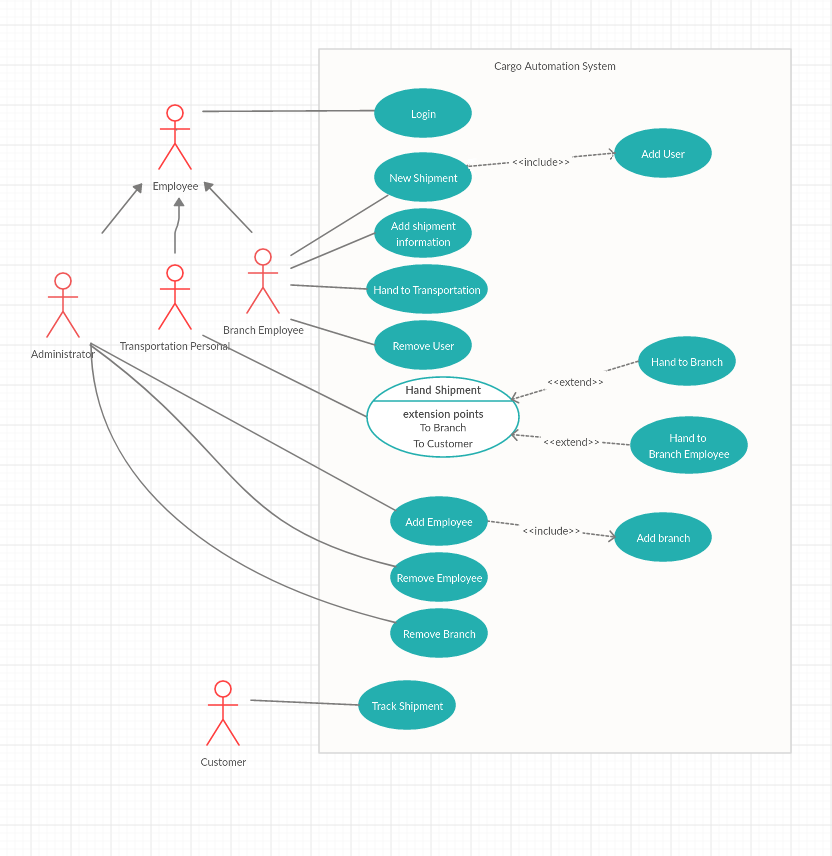
\includegraphics[width=\textwidth]{use-case}
\end{figure}

\newpage

\section{Class Diagrams}

\begin{figure}[htp]
	\centering
	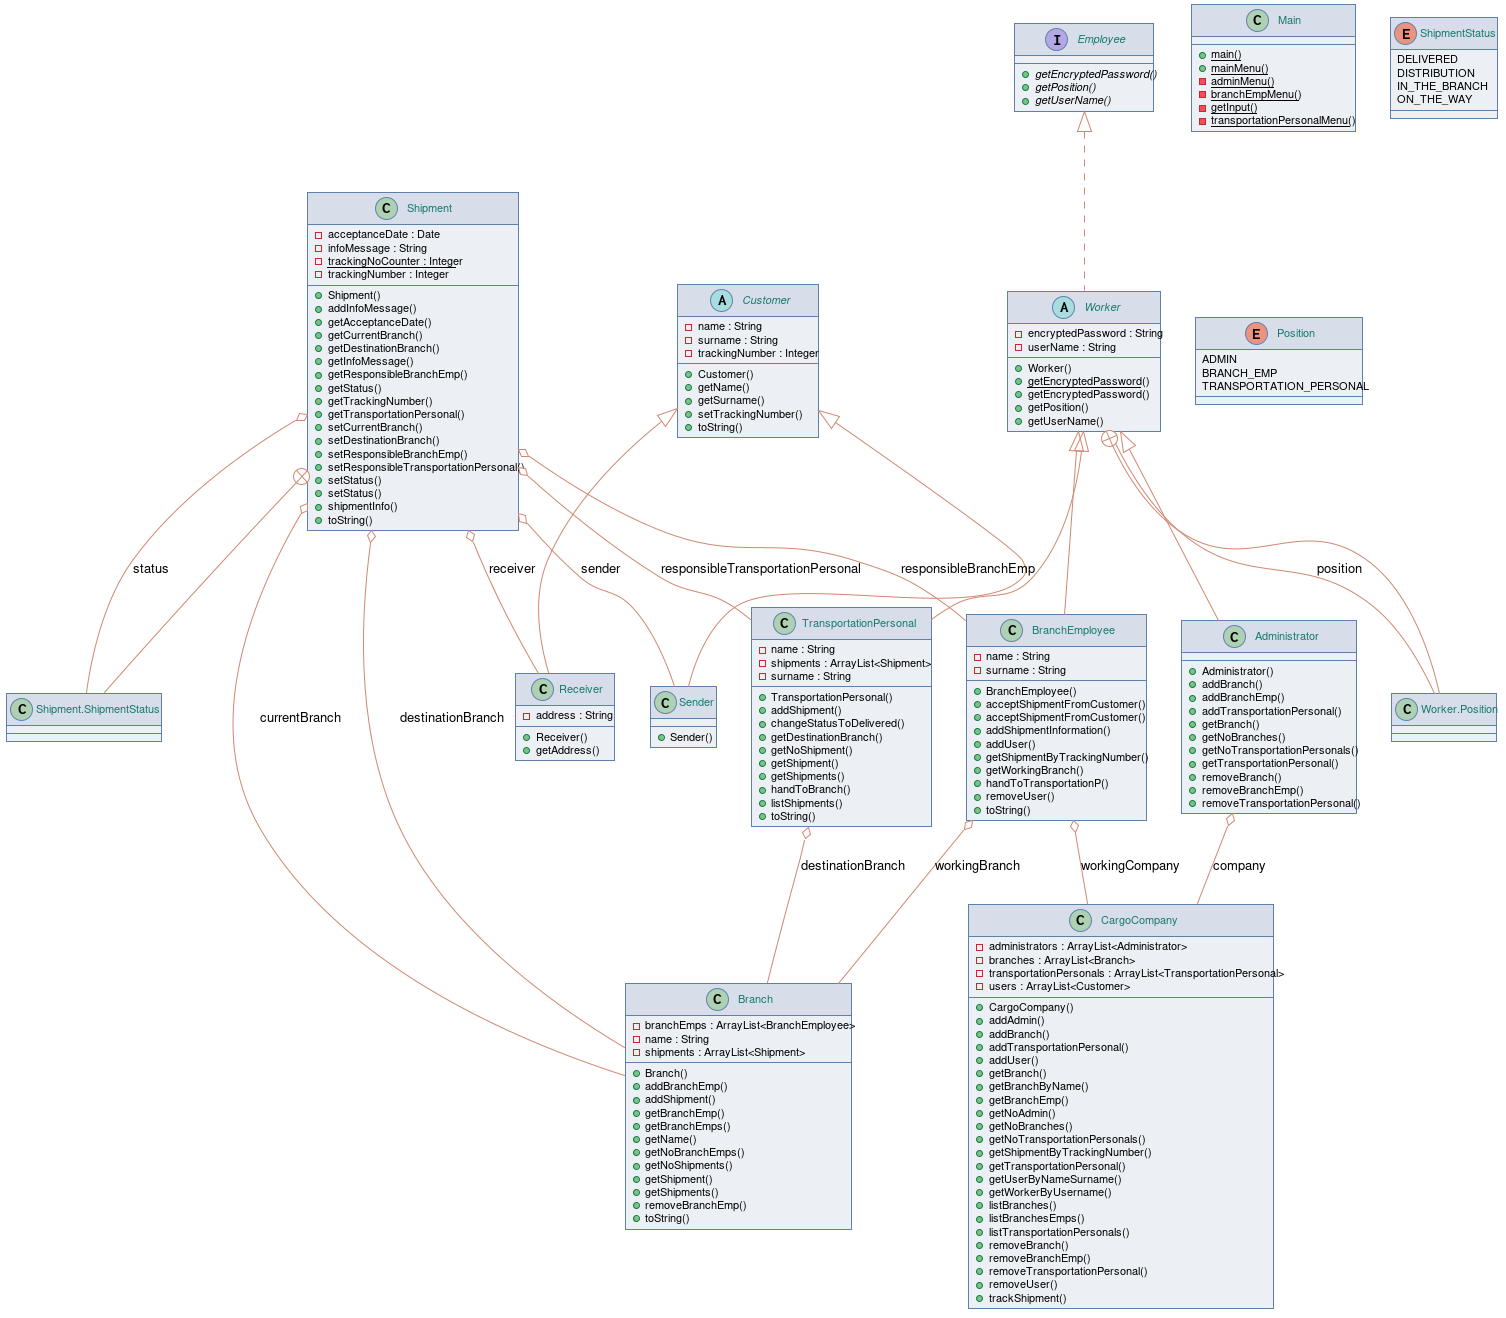
\includegraphics[width=\textwidth]{class-diagram}
\end{figure}

\newpage

\section{Problem Solution Aproach}
The assignment is developing an automation system for a cargo company.
It supposed to be multi-user system. It will be different users and different
tasks they can perform. Also, there are shipments which they have all the
information about its delivery process. Therefore we can treat all these as
set of objects which they have mostly "has a relationship". It's convenient
to use Object Oriented Paradigm.

Since its a good software developing practice, I designed my class
hierarchy by considering encapsulation. However; there will be lots of
classes that need to access the same data. To get over this issue I decided
to create a class (\texttt {CargoCompany}) that stores main data (\texttt {Admins,
Branches, Transportation Personals}).

The program will be used by different users, both user and company
workers. Therefore it would be better to create different classes for users.
Company workers have some common features, so I have created an
abstract class to implement common features.

Another problem I encountered is data needs to be stored and need to be
resized every adding and removing operations. Therefore I used \texttt {ArrayList<...>}, 
since its more convenient to these changings.

The program must be secure in terms of storing user data. So, I store
passwords as encrypted instead of storing them as raw text by concerns of
security. I use the "SHA-256" encryption algorithm in java.security to store
passwords.

I encountered accessing problems from some classes to others, but I
figured it out by creating another object as a field of the first class. And it
makes sense semantically. (\texttt {workingBranch} in \texttt {BranchEmployee},
\texttt {responsibleBranch} in Shipment)

Another issue was creating unique tracking numbers. I used Integer data
type to store tracking numbers, and also used static tracking number
counter value to keep track of the latest tracking number. I also update my
algorithm. When I need to find a shipment by its tracking number I search
through array in reverse order, because latest cargos will be inquired often
compare to older ones.

\newpage

\section{Test Cases}

I tested basic functions of the program in the beginning of main function;

\begin{figure}[htp]
	\centering
	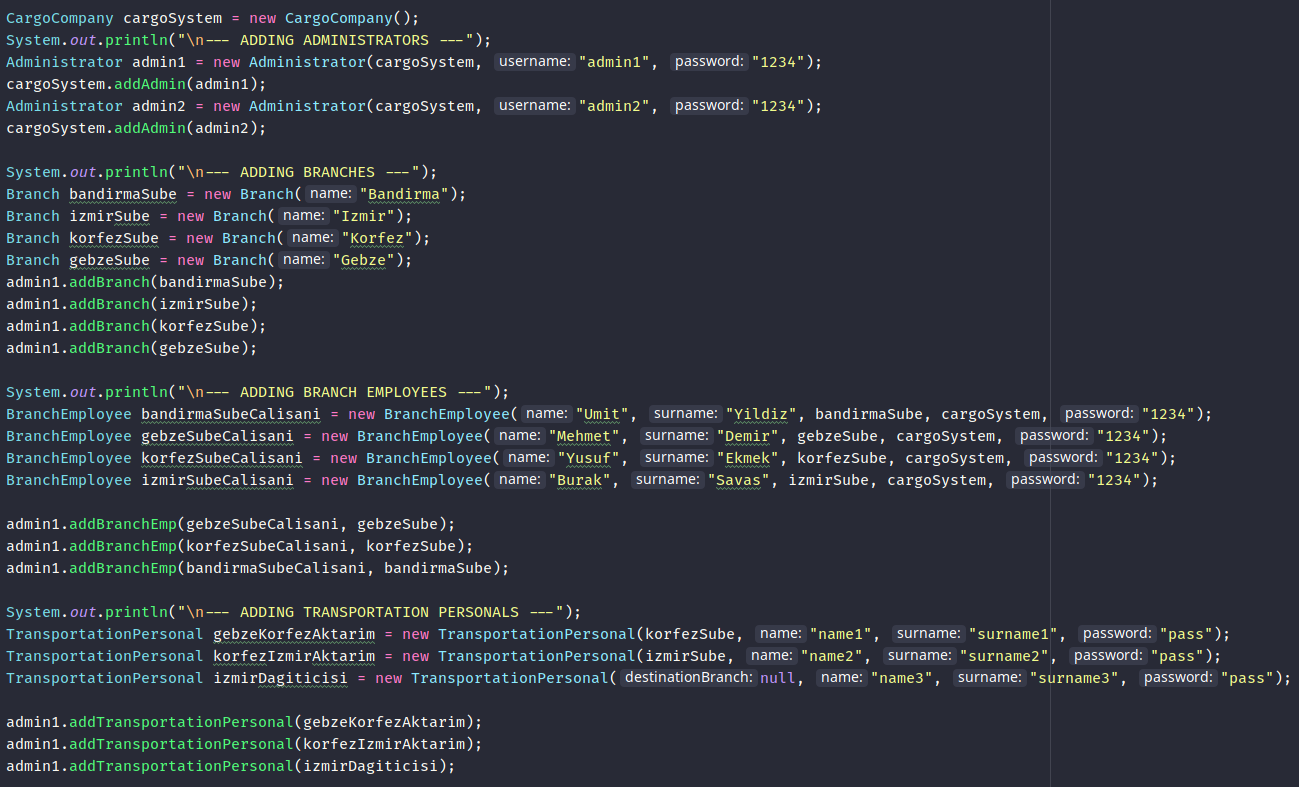
\includegraphics[width=\textwidth]{test-cases-main}
\end{figure}

Terminal output of tested methods after the shipment is delivered;

\begin{center}
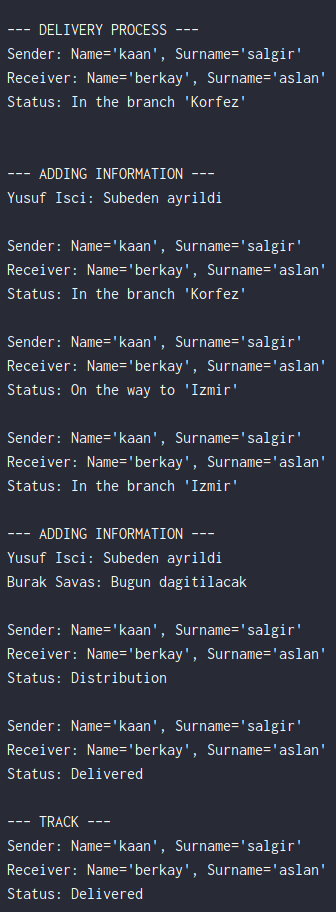
\includegraphics[height=0.45\textheight,keepaspectratio]{test-cases-out}
\end{center}

\newpage

\section{Running and Results}

Caputred screenshots of terminal output of different operations;

\begin{center}

\begin{figure}[htp]
	\caption{Removing branch by administrator}
	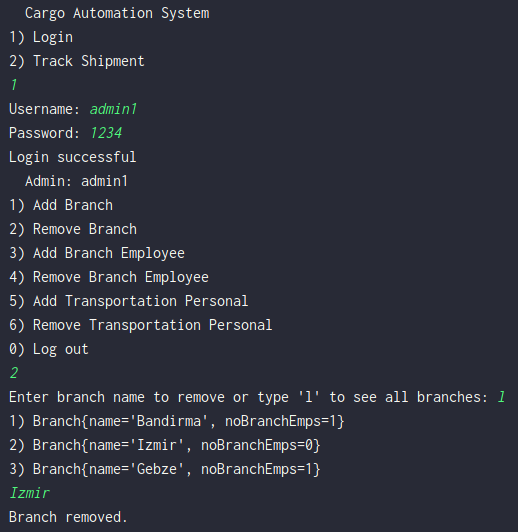
\includegraphics[scale=0.6]{6-1}
\end{figure}
\begin{figure}[htp]
	\caption{Adding new transportation personal}
	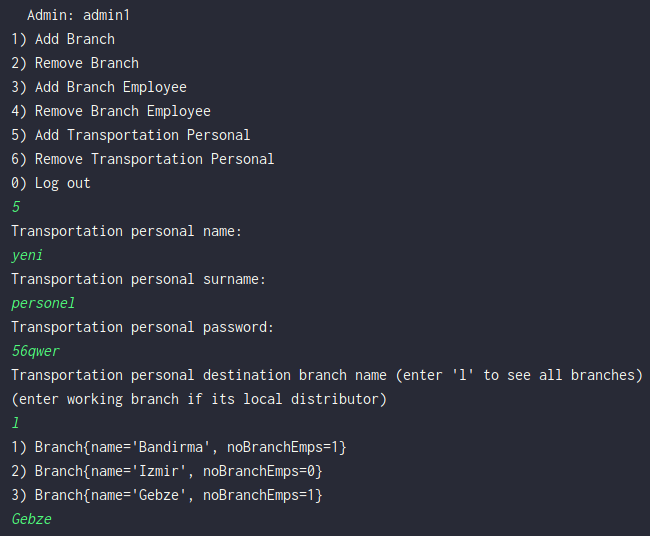
\includegraphics[scale=0.6]{6-2}
\end{figure}
\begin{figure}[htp]
	\caption{Track shipment}
	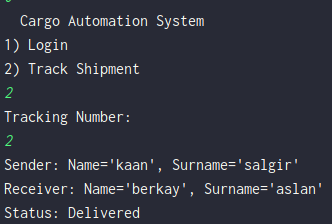
\includegraphics[scale=0.6]{6-3}
\end{figure}
\begin{figure}[htp]
	\caption{Branch employee adds new customer}
	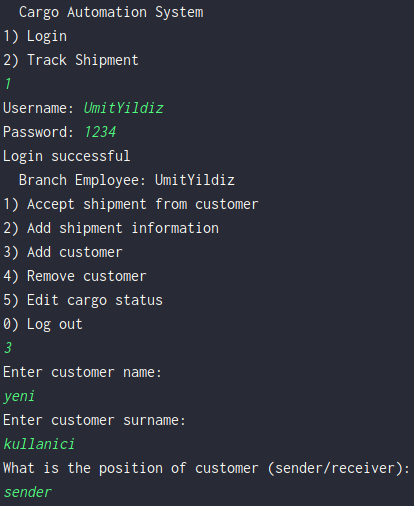
\includegraphics[scale=0.6]{6-4}
\end{figure}
\begin{figure}[htp]
	\caption{Branch employee adds new shipment}
	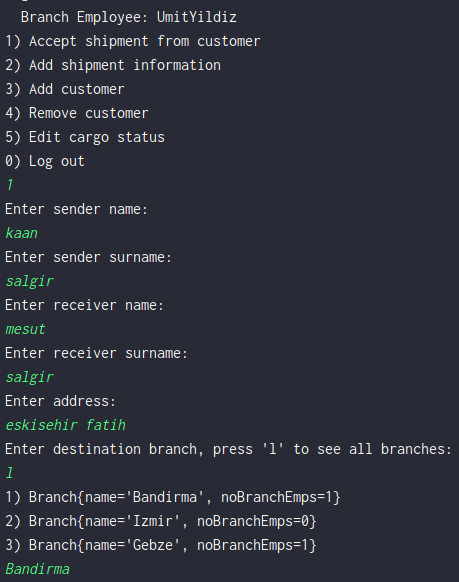
\includegraphics[scale=0.6]{6-5}
\end{figure}

\end{center}
\end{Large}

\end{document}
